% !TEX TS-program = latex
% !TEX root = Thesis_Guo2013.tex

\chapter{Memory Constraints for Power-law Series}
In this Chapter, we will present an application of EPM (\textit{equiprobable partition method}) to time series analysis. With a permutational technique, we will explore the bounds for the 1st-order autocorrelation for series with different (marginal) distributions, including Gaussian, uniform and power-law. 

The 1st-order autocorrelation is a moment defined for multiple variables for characterizing the interdependence among them. Specifically, it can be used to measure the temporal memory effect for time series and it is therefore also referred to as \textit{memory} by some physicists. We found that, very interestingly, for series that follow Gaussian and uniform distributions, the bounds for memory are just the bounds allowed by its definition (natural bounds). However, interestingly, the memory for power-law series is constrained to a much narrower region that relies on the scaling exponent. With EPM, we obtained these bounds when the sample moments involved are divergent, a case that cannot be readily tackled with traditional probabilistic methods. 

\section{Memory for time series}

From a statistical point of view, a time series $ \{t_1, t_2, \cdots, t_n\} $ is a ordered sequence of random variables. Ideally, the distribution for a time series of length $ n $ can be fully characterizes by the joint distribution $ f(t_1, t_2, \cdots, t_n) $. However, for a long series, the space for this distribution is very huge that it can neither be effectively determined or compactly represented. Therefore, we split the characterization for the distribution into two aspects --- the marginal and the interdependence. 

The marginal distribution refers to how one element is distributed regardless of other elements in the series, denoted by $ f(t_1) $, $f(t_2) $, $ \cdots $, $ f(t_n) $. Practically, it is often assumed that the marginal is \textit{stable}, i.e. the marginal distribution for every element is the same and does not change with time. Hence, for example, we can plot all the elements in the series in a histogram and by its distinguished bell curve we learn the marginal is Gaussian. When we speak of Gaussian series or power-law series, we are referring to the marginal distribution.

Aside from the marginal distribution, the elements in the series are intercorrelated by themselves. That is to say, a time series is more than a collection of samples independently drawn from the same marginal. Instead, their temporal ordering affects what values the elements may take. For example, a rising or falling trend is often observed for time series in financial markets. 
And memory (1st-order autocorrelation) is introduced as a simplest measure to characterize the interdependence among these elements \cite{Goh2008}. 

For a time series $ \{t_1, t_2, \cdots, t_{n}\} $, memory is defined as the Pearson's correlation coefficient between $ \{t_{2}, t_{3}, \cdots, t_{n} \}$ and its lag-1 counterpart $ \{t_{1}, t_{2}, \cdots, t_{n-1}\} $, i.e.
\begin{equation}
	M = \frac{1}{n-1} \sum_{i=1}^{n-1} \frac{(t_i - m_1)(t_{i+1} - m_2)}{\sigma_1 \sigma_2},
\end{equation}
where $ m_1, m_2 $  and $ \sigma_1, \sigma_2 $ refer to the mean and standard deviation of the two series. Intuitively from the definition, memory describes the temporal \textit{consistency} of a series: if a big (compared to average) element tends to follow a big element and a small one tends to follow a small one, then the series is \textit{consistent} and its memory is positive; on the contrary, if a big one tends to follow a small one and a small one tends to follow a big one, then the series is \textit{inconsistent} and its memory is negative. 

Due to Cauchy-Schwartz inequality
\begin{equation}
	\left\vert M \right\vert \leq \frac{1}{\sigma_1 \sigma_2} \sqrt{\left[ \frac{1}{n-1} \sum_{i=1}^{n-1} (t_i - m_1)^2  \right] \left[ \frac{1}{n-1} \sum_{i=1}^{n-1} (t_{i+1} - m_2)^2 \right]} = 1,
\end{equation}
the natural bounds $ -1 \leq M \leq 1 $ hold for all series. The upper extreme $ +1 $ marks the maximum consistency and the minimum $ -1 $ marks the power extreme $ -1 $ marks the minimum consistency. And $ M=0 $ suggests that the series is neither consistent or inconsistent --- the series is similar to independently samples in this regard and the short-range interdependence among elements is weak.

\section{Modeling correlated series with a specified marginal}
Clearly, when every $ t_{i} $ is independently sampled from the same marginal distribution $ f(x) $ , there is no interdependence among elements and the expectation value of $ M $ is zero. To modify the interdependence structure while preserving the marginal, we first sort the independently sampled series and then reorder the samples by a permutation $ \theta $ with regard to every element's ranking in the sorted series.
The sorted series directly give us the order statistics $ \{t_{(i)}\} $, 
where $ 0 < t_{(1)} \leq t_{(2)} \leq \cdots \leq t_{(n)} $.  
Then, by applying a permutation $ \theta $ (a one-to-one mapping from the set $ \{1, 2, \cdots, n\} $ to itself) to $ \{t_{(i)}\} $, we now have a sequence $ \{t_{(\theta_{i})}\} $ with a different interdependence structure but the same marginal marginal distribution. 

For a series samples from a specified marginal, by changing $ \theta $, i.e. the way we permute them, we can expect series produced with different values of memory $ M $. For example, if series are permuted such that big elements tend to be followed by big ones and small followed by small ones, $ M $ would be positive; on the contrary, if big elements followed by small ones and small elements followed by big ones, $ M $ would be negative. 

\subsection{Permutational extremes for memory}
Interestingly, there exist fixed $ \theta_{\max} $ and $ \theta_{\min} $ that respectively maximizes and minimizes $ M $ among all possible permutations. And we can use these two extremes to derive the bounds for memory in the sense of all permuted independent samples.

To see this, we need to find out how a permutation affects $ M $. 
As the values of the two aforementioned series are different in only one element ($ t_{1} $ in head and $ t_{n} $ in tail), we assume $ m_{1} = m_{2} = m$ and
$ \sigma_{1} = \sigma_{2} = \sigma $ when $ n $ is large, where $ m $ and $ \sigma $ are the mean and standard deviation of the whole series. Then the memory  of $ \{t_{(\theta_i)}\} $ can be rewritten as
\begin{equation}
	M = \frac{1}{\sigma^2} \big( \frac{1}{n-1} \sum_{i=1}^{n-1} t_{(\theta_i)}t_{(\theta_{i+1})} - m^2 \big), \label{eqs:MSimple}
\end{equation} 
where the reordering of the series only affects the summed products of adjacent terms $ S_{\theta} = \sum_{i=1}^{n-1} t_{(\theta_i)} t_{(\theta_{i+1})} $, while leaving $ m $ and $ \sigma $ unchanged. The desired extreme permutations for $ M $ are just those maximize/minimizes $ S_{\theta} $, denoted by $ \theta_{\max} $ and $ \theta_{\min} $. It has been shown that, for any $ n $,  there are fixed $ \theta_{\max} $ and $ \theta_{\min} $ for any real numbers $ t_{(1)} \leq t_{(2)} \leq \cdots \leq t_{(n)} $ \cite{Hallin1992} \footnote{Whereas \cite{Hallin1992} uses an objective function that sums the products in a circle, i.e. $S^{\prime}_{\theta} = \sum_{i=1}^{n-1} t_{\theta_{i}} t_{\theta_{i+1}} + t_{\theta_{1}} t_{\theta_{n}}$, the results can be reduced to our case by introducing an additional $ S_0 = 0 $ to the series, which makes zero contribution to the sum.}.

$ \theta_{\max} $ obtains the maximum memory by first arranging the odd elements of order statistics in the increasing order, followed by even elements in the decreasing order, which is
\begin{equation}
\begin{split}
&t_{(1)}, t_{(3)}, \cdots, t_{(2l-1)}, t_{(2l)}, t_{(2l-2)}, \cdots, t_{(4)}, t_{(2)} \quad (n=2l), \\
&t_{(1)}, t_{(3)}, \cdots, t_{(2l-1)}, t_{(2l+1)}, t_{(2l)}, \cdots, t_{(4)}, t_{(2)} \quad (n=2l+1). \\
\end{split} \label{eqs:maxArrange}
\end{equation} 
For simplicity, we only address the case when $ n=2l $, the sum with order statistics is expressed as 
\begin{equation}
	S_{\theta_{\max}} = \sum_{i=1}^{2l-2} t_{(i)}t_{(i+2)} + t_{(2l)}t_{(2l-1)} \quad (n=2l), \label{eqs:Smax}
\end{equation}
while the case of odd $ n $ can be handled similarly.



 
On the contrary, $ \theta_{\min} $ arranges the order statistics by alternating small and big terms, i.e.
\begin{equation}
\begin{split}
&t_{(2l)}, t_{(1)}, t_{(2l-2)}, \cdots, t_{(2l-3)}, t_{(2)}, t_{(2l-1)} \quad (n=2l), \\
&t_{(2l)}, t_{(2)}, \cdots, t_{(l)}, \cdots, t_{(1)}, t_{(2l+1)} \quad (n=2l+1).
\end{split} \label{eqs:minArrange}
\end{equation}
Again, for even $ n $, we have
\begin{equation}
	S_{\theta_{\min}} = \sum_{i=1}^{l-1} \big( t_{(i)}t_{(2l+1-i)} + t_{(i)}t_{(2l-1-i)} \big) + t_{(l)}t_{(l+1)} \quad (n=2l).
\end{equation}

We then define the upper bound and lower bound for memory as the mathematical expectation of $ M $ under $ \theta_{\max} $  and $ \theta_{\min} $ respectively. And in the limit of large length of series, the bounds 
\begin{equation}
M_{\max} = \lim_{n \rightarrow \infty}\E{[M(t_{\theta_{\max}})]}
\end{equation}
and
\begin{equation}
M_{\min} = \lim_{n \rightarrow \infty}\E{[M(t_{\theta_{\min}})]}
\end{equation}
can be derived in a closed form or effectively approximated. It can be shown that $ M_{\max}=1 $ and $ M_{\min}=-1 $ hold for Gaussian and uniform distributions, corresponding the natural range of $ M $. However, a much narrower range is found for power-law distributions, where the bounds rely on the exponent $ \alpha $. It shall be noted that the bounds discussed here are tight as they are the values of $ M $ under permutations $ \theta_{\max} $ and $ \theta_{\min} $.

\section{The bounds for memory}
\subsection{Adjusting memory by iterative rearrangement}
Before an in-depth theoretical treatment, we first explore the bounds for uniform, Gaussian and power-law samples by iteratively rearranging them towards $ \theta_{\max} $ or $ \theta_{\min} $. 

To do this, we construct an approximation of the order statistic iteratively. The process contains $ n $ steps, the same as the length of the series. In each step, the series is rearranged with one pass of bubble sort on the series produced after the last step, which means stepping through the series from the first element to the last, comparing each pair of adjacent elements and swap them if they are not in increasing order. The series obtained after $ i $ such steps is denoted as $ \{ \tilde{t}^{(i)} \} $, as an approximation to the order statistics, with $ \{ \tilde{t}^{(n)} \} $ guaranteed to be the same as the order statistics because a bubble sort always finishes in $ n $ passes.

In each step, treating $ \{ \tilde{t}^{(i)} \} $ as approximate order statistics, series with positive and negative memory are obtained by rearranging $ \{ \tilde{t}^{(i)} \} $  according to (\ref{eqs:maxArrange}) and (\ref{eqs:minArrange}) respectively.

In our experiment, series are of length $ n=10,000 $, independently drawn from uniform distribution on $ [0,1] $, standard Gaussian distribution (all samples are added by the same positive constant afterwards to ensure being positive), and power-law distribution whose probability density function is
\begin{equation}
	f(t) = \frac{\alpha-1}{t_{\min}} (\frac{t}{t_{\min}})^{-\alpha},
\end{equation}
with $ t_{\min}=1 $ and $ \alpha=3.5 $.
Results are obtained by averaging 5 independent runs and reported by Figure \ref{fig:TuningUpMem} for positive memory and Figure \ref{fig:TuningDownMem} for negative memory.

\begin{figure}[!ht]
\centering
\includegraphics[width=0.7\textwidth]{figures/TuningUp-power-uni-gauss.eps}
\caption{Memory tuned up by iteratively rearranging independently sampled series.}
\label{fig:TuningUpMem}
\end{figure}

\begin{figure}[!ht]
\centering
\includegraphics[width=0.7\textwidth]{figures/TuningDown-power-uni-gauss.eps}
\caption{Memory tuned down by iteratively rearranging independently sampled series.}
\label{fig:TuningDownMem}
\vspace{1em}
\end{figure}


As can be seen, by rearranging the series towards $ \theta_{\max} $, 
the memory goes to $ +1 $ for all three distributions. 
As is noted, the maximum memory of power-law series after the last iteration is slightly below $ +1 $, 
due to the effect of finite $ n $, which we will see later. 
However, while the memory can be tuned down to $ -1 $ by rearrangement towards $ \theta_{\min} $  for uniform and Gaussian distributed series, 
it is bounded above about $ -0.2 $ for the power-law series. 
In the following sections, we will further analyze how this non-trivial lower bound depends on the exponent $ \alpha $.
\subsection{Probablistic method for the $ \alpha>3 $ case}
To derive how the bounds rely on $ \alpha $, we first consider the case where $ \alpha > 3 $, which is necessary for the population variance $ \sigma({\alpha})^{2} $ to converge, and the corresponding sample variance $ \sigma^{2} $ appear in the denominator of $ M $. When $ \alpha>3 $, by simply equating the sample moments with the corresponding population moments, we have 
\begin{equation}
	\E[M(t_{\theta})] = \frac{1}{\sigma(\alpha)^2} (\frac{1}{n-1} \sum_{i=1}^{n-1} \E[t_{\theta_i}t_{\theta_{i+1}}] -m(\alpha)^2 ), \label{eqs:Mprob}
\end{equation} 
where
\begin{equation}
	m(\alpha) = \int_{1}^{+\infty} xf(x) dx = \frac{\alpha-1}{\alpha-2},
\end{equation}
\begin{equation}
	\sigma(\alpha)^2 = \int_{1}^{+\infty} x^{2}f(x) dx - m(\alpha)^{2} = \frac{\alpha-1}{\alpha-3} - m(\alpha)^2.
\end{equation}
Here, $ f(x) = (\alpha-1)x^{-\alpha} $ is the PDF for power-law, and without loss of generality, we assume $ x_{\min}=1 $ because $ M $ would remain the same if every $ t_{i} $ is divided by the same constant.

The upper bound directly relates to $ \lim_{n \rightarrow \infty} \frac{1}{n-1} E[S_{\theta_{\max}}] $, 
where the expected value of $ S_{\theta_{\max}} $ is composed of the expected value of products of adjacent items according to equation (\ref{eqs:Smax}), i.e.
\begin{equation}
	\frac{1}{n-1}\E[S_{\theta_{\max}}] = \frac{1}{2l-1}\sum_{i=1}^{2l-2} \E[t_{(i)} t_{(i+2)}] + \frac{1}{2l-1} \E[t_{(2l)} t_{(2l-1)}], \label{eqs:s-maxmem}
\end{equation}
assuming $ n=2l $. The case when $ n=2l+1 $ can be worked out in a similar fashion to arrive at the same results.

The expected value of each term can be obtained by using the joint distribution of order statistics. 
The probability density function for the joint distribution of two order statistics $ t_{(j)}, t_{(k)}\  (j <k)$ is given by \cite{David2003}
\begin{equation}
	f_{t_{(j)}, t_{(k)}} (x,y) = n! \frac{[F(x)]^{j-1}}{(j-1)!} \frac{[F(y) - F(x)]^{k-1-j}}{(k-1-j)!} \frac{[1-F(y)]^{n-k}}{(n-k)!} f(x) f(y) \quad  (x \leq y),
\end{equation}
where $ F(x) $ is the cumulative distribution function for power-law, i.e.
\begin{equation}
	F(x) = \int_{x}^{+\infty}f(u)du = 1 - x^{1-\alpha}.
\end{equation}
Therefore, we have
\begin{equation}
\begin{split}
	\E[t_{(i)} t_{(i+2)}] &= \iint_{1 \leq x \leq y < \infty} x y f_{t_{(i)}, t_{(i+2)}}(x,y) dx dy \\
	&= \frac{\Gamma(2l+1)}{\Gamma(2l+1-2c)} \frac{\Gamma(2l-i+1-2c)}{\Gamma(2l-i-1)} \frac{1}{[(2l-i) - c][(2l-i) - \alpha c]} \quad (1 \leq i \leq 2l-2),
\end{split}
\end{equation}
and
\begin{equation}
\begin{split}
\E[t_{(2l-1)}t_{(2l)}] &= \iint_{1 \leq x \leq y < \infty} x y f_{t_{(2l-1)}, t_{(2l)}}(x,y) dx dy \\
&= \frac{(\alpha-1)^2}{2(\alpha-2)^2} \Gamma(3-2c) \frac{\Gamma(2l+1)}{\Gamma(2l+1-2c)},
\end{split}
\end{equation}
where we use a shorthand $ c = \frac{1}{\alpha-1}$ ($ 0<c<\frac{1}{2} $).

In the limit of $ n \rightarrow \infty $, the first term in (\ref{eqs:s-maxmem}) would be
\begin{equation}
\begin{split}
	&\quad \lim_{l \rightarrow \infty} \frac{1}{2l-1} \sum_{i=1}^{2l-2} E[t_{(i)} t_{(i+2)}] \\
	&= \lim_{l \rightarrow \infty} \frac{1}{2l-1} \frac{\Gamma(2l+1)}{\Gamma(2l+1-2c)} \sum_{i=1}^{2l-2} \frac{1}{[2l-i-2c][2l-i-\alpha c]} \frac{\Gamma(2l-i+1-2c)}{\Gamma(2l-i-1)}.
\end{split}
\end{equation}
Reducing the prefactor by using a property of Gamma function, namely
\begin{equation}
	\lim_{x \rightarrow \infty} \frac{\Gamma(x)}{\Gamma(x+\gamma) x^\gamma} = 1 \ \text{for real}\ \gamma,
\end{equation}
and rewriting the summation with index $ k = 2l - i $, we have
\begin{equation}
\quad \lim_{l \rightarrow \infty} \frac{1}{2l-1} \sum_{i=1}^{2l-2} E[t_{(i)} t_{(i+2)}] = \lim_{l \rightarrow \infty} (2l+1)^{-(1-2c)} \sum_{k=2}^{2l-1} \frac{1}{(k-c)(k-c-1)} \frac{\Gamma(k+1-2c)}{\Gamma(k-1)}.
\end{equation}
As $ c < \frac{1}{2} $, the prefactor approaches zero when $ n \rightarrow \infty $, 
making the result depends on the limiting behavior of the summing terms only. Now we have
\begin{equation}
\quad \lim_{l \rightarrow \infty} \frac{1}{2l-1} \sum_{i=1}^{2l-2} E[t_{(i)} t_{(i+2)}] = \lim_{l \rightarrow \infty} \sum_{k=2}^{2l-1} (\frac{k}{2l+1})^{-2c} \frac{1}{2l+1} = \int_{0}^{1} t^{-2c} dt = \frac{\alpha-1}{\alpha-3}. \label{eqs:s1-maxmem}
\end{equation}
Meanwhile, the second term in the RHS of (\ref{eqs:s-maxmem}) vanishes in the limit of large $ n $, i.e.
\begin{equation}
	\lim_{l \rightarrow \infty} \frac{1}{2l-1} \E[t_{(2l)} t_{(2l-1)}] = 0. \label{eqs:s2-maxmem}
\end{equation}
Substituting (\ref{eqs:s1-maxmem}) and (\ref{eqs:s2-maxmem}) into (\ref{eqs:Mprob}), we arrive at 
\begin{equation}
	M_{\max} = \lim_{n \rightarrow \infty} \E[M_{\theta_{\max}}] = 1 \quad (\alpha>3). \label{eqs:max-mem-theory}
\end{equation}

Similarly, to obtain the lower bounds, we rewrite the summed products as 
\begin{equation}
	 \frac{1}{n-1} \E[S_{\theta_{\min}}] = \frac{1}{2l-1} \sum_{i=1}^{l-1} \left(\E[t_{(i)} t_{(2l+1-i)}] + \E[t_{(i)} t_{(2l-1-i)}] \right) + \frac{1}{2l-1} \E[t_{(l)}t_{(l+1)}],
\end{equation}
again assuming $ n=2l $ for convenience.
Taking the large $ n $ limit, we have
\begin{equation}
\begin{split}
&\quad \lim_{l \rightarrow \infty} \frac{1}{2l-1} \sum_{i=1}^{l-1} \E[t_{(i)} t_{(2l+1-i)}] \\
&= \lim_{l \rightarrow \infty} \frac{1}{2l-1} \frac{\Gamma(2l+1)}{\Gamma(2l+1-2c)} \sum_{i=1}^{l-1} \frac{\Gamma(i+2-c)}{\Gamma(i+2)} \frac{\Gamma(2l-i+1-2c)}{\Gamma(2l-i+1-c)} \\
&= \lim_{l \rightarrow \infty} (2l+1)^{-(1-2c)} \sum_{i=1}^{l-1} (i+2)^{-c} (2l-i+1)^{-c} \\
&= \lim_{l \rightarrow \infty} \sum_{i=1}^{l-1} (\frac{i+2}{2l+1})^{-c} (1-\frac{i}{2l+1})^{-c} (\frac{1}{2l+1}) \\
&= \int_{0}^{\frac{1}{2}} u^{-c} (1-u)^{-c} du \\
&= B(\frac{1}{2}; \frac{\alpha-2}{\alpha-1}, \frac{\alpha-2}{\alpha-1}),
\end{split}
\end{equation}
where $ B $ is the \textit{incomplete beta function}, defined as 
\begin{equation}
	B(x; a,b) = \int_{0}^{x} t^{a-1} (1-t)^{b-1} dt.
\end{equation}
We also have the other term with the same limit, namely 
\begin{equation}
\lim_{l \rightarrow \infty} \frac{1}{2l-1} \sum_{i=1}^{l-1} \E[t_{(i)} t_{(2l-1-i)}] = B(\frac{1}{2}; \frac{\alpha-2}{\alpha-1}, \frac{\alpha-2}{\alpha-1}),
\end{equation}
and again the remaining term vanishes in the limit, i.e.
\begin{equation}
	\lim_{l \rightarrow \infty} \frac{1}{2l-1} \E[t_{(l)}t_{(l+1)}] = 0.
\end{equation}
Therefore, the minimum memory is derived as
\begin{equation}
	M_{\min} = \lim_{n \rightarrow \infty} \E[M_{\theta_{\min}}] = \frac{1}{\sigma(\alpha)^2} \left[ 2B\left(\frac{1}{2}; \frac{1}{m(\alpha)}, \frac{1}{m(\alpha)}\right)  - m(\alpha)^2\right] \quad(\alpha>3). \label{eqs:min-mem-theory}
\end{equation}

\subsection{EPM approximations for the $ \alpha<3 $ case}
Having obtained the upper bound \label{eqs:max-mem-theory} and the lower bound\label{eqs:min-mem-theory} for $ \alpha>3 $, we now turn to the case for $ 1 < \alpha \leq 3 $ ($ \alpha > 1$ is necessary for power-law to be normalized). In this case, the corresponding population moment for $ \sigma^{2} $ would diverge ($ m(\alpha) $ also diverges when $ \alpha <2 $), rendering the moment-substitution technique infeasible. Meanwhile, the probability distributions of $ M(t_{\theta_{\max}}) $ and $ M(t_{\theta_{\min}}) $ themselves are intractable. Therefore, we present an approximation method that recovers the asymptotic behavior of statistics when $ n \rightarrow \infty $ by substituting random variables with determinant values. 

To do so, we pick the points $ \{\hat{t}_1, \hat{t}_2, \cdots, \hat{t}_n\} $ that cut the area under the probability density function $ f(t) $ into slices of equal area $ \frac{1}{n} $, with $ \hat{t}_1 = x_{\min} = 1 $ and the area from $ t_{n} $ extending to infinity also being $ \frac{1}{n} $. Then we approximate the random samples $ \{ t_{(1)}, t_{(2)}, \cdots, t_{(n)} \} $  with these determinant points $ \{ \hat{t}_1, \hat{t}_2, \cdots, \hat{t}_n \} $. It should be noted that such approximation imposes a cut-off on the maximum value of $ \{t_i\} $ and the probability of drawing a sample exceeding the cut-off is $ \frac{1}{n} $ , which diminishes to zero as $ n \rightarrow \infty $.    
By setting $ \int_{1}^{\hat{t}_i} = \frac{i-1}{n} $, we have
\begin{equation}
	\hat{t}_i = (1-\frac{i-1}{n})^{-c}  \quad (i=1,2,\cdots,n),
\end{equation}
where $ c = \frac{1}{\alpha-1} > \frac{1}{2} $ in this case. 

Rewriting $ M $ in terms of samples as
\begin{equation}
\begin{split}
	M = \frac{s-m^{2}}{\overline{t^{2}} -m^{2}},
\end{split}	
\end{equation} 
where $ s = \frac{1}{n-1} S = \frac{1}{n-1} \sum_{i=1}^{n-1} t_{i} t_{i+1}$, $ \overline{t^2} = \frac{1}{n} \sum_{i=1}^n t_i^2 $ and $ m^2 = (\frac{1}{n}\sum_{i=1}^n t_i)^2 $ are the statistics in concern. By substituting $t_{(i)}$ with $ \hat{t}_i $, we seek approximations for these statistics in the form of $ n^{\mu(\alpha)}g(n,\alpha) $, where when $ n \rightarrow \infty $, $ g(n,\alpha) $ converges to a function of $ \alpha $ while the divergence is characterized by the term $ n^{\mu(\alpha)} $.

Then, for the upper bound, we have
\begin{equation}
\hat{s}_{\theta_{\max}} = \frac{n^{2c}}{n-1} \big[ \sum_{k=2}^{n-1} (k^2-1)^{-c} + 2^{-c} \big]
\end{equation}
and
\begin{equation}
\overline{{\hat{t}}^2}_{\theta_{\max}} = \frac{1}{n} \sum_{i=1}^{n} \hat{t}_i^2 = n^{2c-1} \sum_{k=0}^{n-1} (k+1)^{-2c} ,
\end{equation}
both of which diverge with the order of $ n^{2c-1} $, while it is found that $ \hat{m}^2 $ either converges when $ 2 < \alpha \leq 3$ or diverges with a lower order $ n^{2c-2} $ when $ 1 < \alpha \leq 2 $. Hence, in the limit of large $ n $, $ M_{\theta_{\max}} $ can be approximated by neglecting $ \hat{m}^2 $. Therefore, we have
\begin{equation}
\begin{split}
	M_{\max} &\approx \lim_{n \rightarrow \infty} \hat{M}_{\theta_{\max}} = \lim_{n \rightarrow \infty} \frac{\sum_{k=2}^{n-1} (k^2-1)^{-c} + 2^{-c}}{\sum_{k=0}^{n-1} (k+1)^{-2c}} \quad (c=\frac{1}{\alpha-1},\ 1 < \alpha \leq 3),
\end{split} \label{eqs:mmax-approximate-theory}
\end{equation}
where both the numerator and the denominator are convergent and can thus be approximately computed by taking a large $ n $. 

Meanwhile, when analyzing the lower bound with the same method, it is found that 
$ \overline{{\hat{t}}^2}_{\theta_{\min}} $ is the term diverging with the biggest order of $ n $, while the orders for $ \hat{m}^2 $ and $ \hat{s}_{\theta_{\min}} $ are smaller if they diverge. Because the term with the biggest order only appears in the denominator, we have
\begin{equation}
	M_{\min} \approx \lim_{n \rightarrow \infty} \hat{M}_{\theta_{\min}} = 0.
\end{equation}

\begin{figure}[!h]
\begin{center}
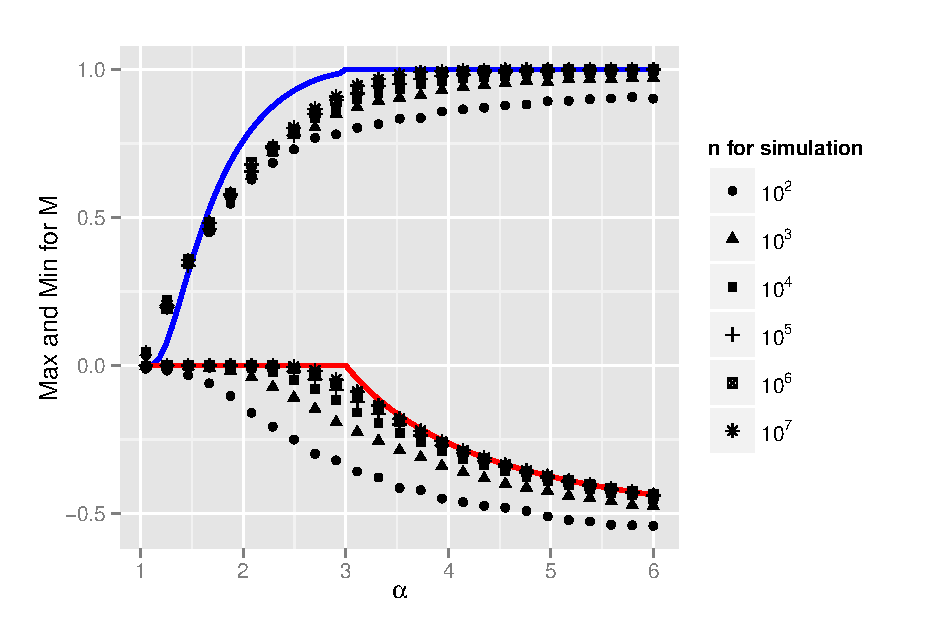
\includegraphics[width=0.9\columnwidth]{figures/ch3_limitedSysSizeEffect.eps}
\caption{Theoretical bounds for $ M_{\min} $ and $ M_{\max} $ and numerical simulations with different series lengths. Each point in simulation is produced by averaging 1000 independent runs.}
\label{fig:limitedSysSize}
\end{center}
\end{figure}
To summarize, as shown by the solid curves in Fig. \ref{fig:limitedSysSize}, when $ \alpha $ grows from 1 to 3, the lower bound remains 0 while the upper bounds increases from 0 to +1, constraining $ M $ to the positive region; when $ \alpha $ grows above 3, the upper bound remains +1 while the lower bound slides down to the negative region as a decreasing function of $ \alpha $, but with the limit $ M_{\min} \rightarrow -0.64 \ (\alpha \rightarrow \infty) $. Fig. \ref{fig:limitedSysSize} also reports the numerical values of $ M_{\min} $ and $ M_{\max} $ of series with finite lengths, produced by drawing independent samples and permuting them by $ \theta_{\min} $ and $ \theta_{\max} $. The gap resulted from finite system size diminishes with larger $ n $. 

\section{Empirical studies}
We study the distribution of memory against the scaling exponent from empirical time series data that follow power-law distributions. To this end, we use \textit{inter-event time series} data collected from online human activities. Inter-event time series refer to the series made up of time intervals between consecutive events and have been widely found to follow power-law distributions. 

The \textit{Movielens} dataset collects the time stamps for the users on its website\footnote{www.movielens.org} when they make a rating for movies. Then, one user corresponds to one inter-event time series, which is composed of time intervals between every two consecutive ratings. And the \textit{Twitter} dataset collects the time stamps when users send a tweet. Then the inter-event time series for a user is made up of time intervals between every two tweeting actions of him or her.

Because the datasets do not explicitly contain the parameters for power-law, we estimate the scaling exponent $ \alpha $ with the MLE method proposed by \cite{Clauset2009}. As we are examining the property of long power-law series, we rule out those series that are either too short ($ n<190 $)  or are unlikely to follow a power-law ($ p-value<0.1 $). $ p-value $ is used as a goodness-of-fit test based on the Kolmogorov-Smirnov (KS) statistic and likelihood ratios, which is also suggested by \cite{Clauset2009}.


\begin{figure}[!h]
\begin{center}
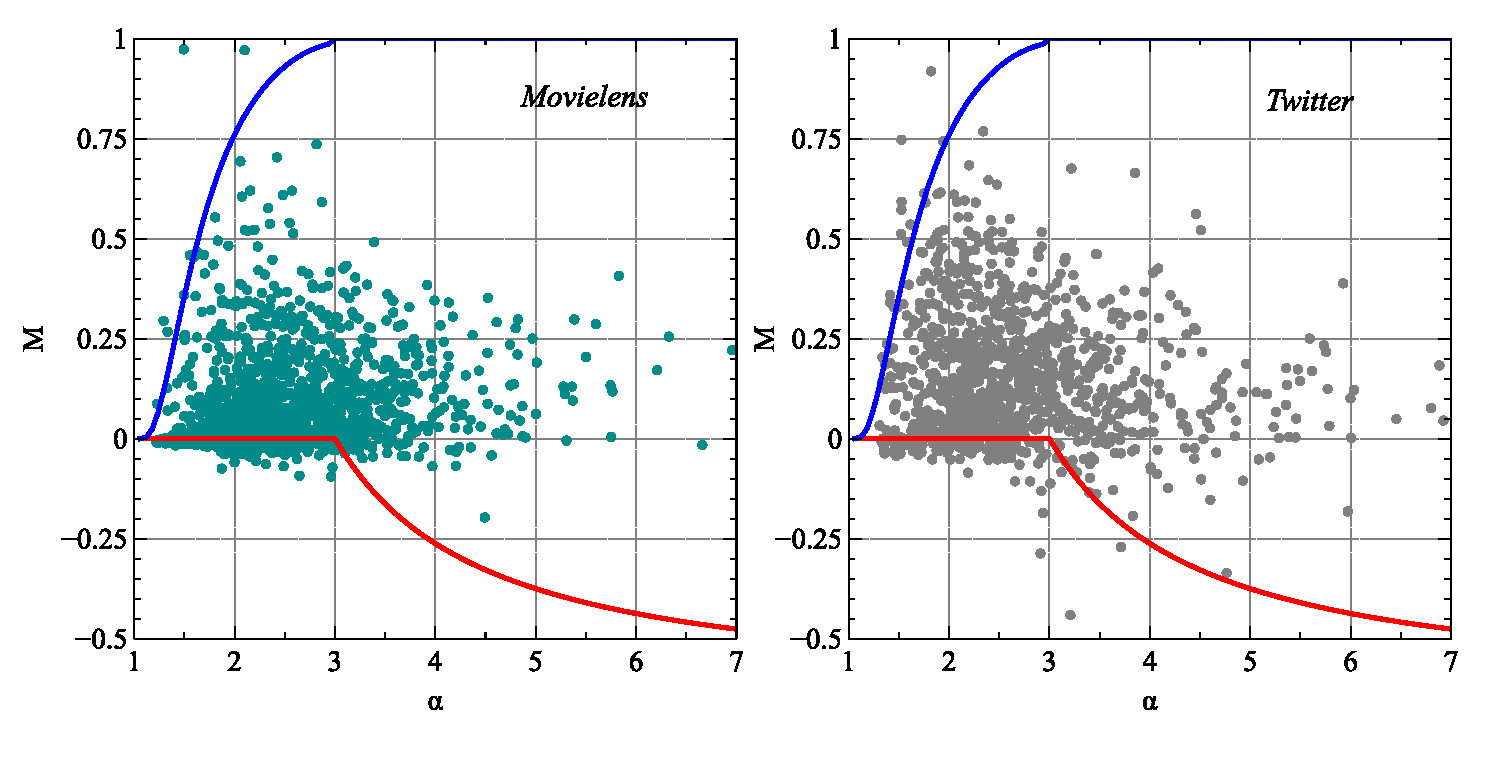
\includegraphics[width=0.95\textwidth]{figures/ch3_empirical_mem.eps}
\caption{Memory for power-law distributed inter-event time series from empirical inter-event time series, where each series is represented by a point and theoretical bounds are drawn as solid curves. The regions of memory from empirical data agree with theoretical bounds. Left: \textit{MovieLens} dataset for online movie rating. Right: \textit{Twitter} dataset for sending tweets. }
\label{fig:movlens}
\end{center}
\end{figure}
In agreement with theoretical values, we find the memory constraints existing in empirical power-law data. Fig. \ref{fig:movlens} plots $(\alpha, M)$ for power-law distributed inter-event time series selected from the \textit{MovieLens} dataset and the \textit{Twitter} dataset. Data points in both datasets fall into the regions predicted by theoretical bounds. A few outliers are either due to the last interval being exceptionally large (beyond the upper bounds) or the fact that they are programmed robots that perform actions at fixed times (beyond the lower bound).






